
\section{Einleitung zu den Klassendiagrammen}
In der Web-Application benutzen wir Typescript um in Javascript Typsicherheit zu gewähren. In den Diagrammen werden deshalb Typescript spezifische Typen und Utility Typen benutzt. Hierfür siehe Typescript Docs für Advanced Types und Utility Types: \\
\url{http://www.typescriptlang.org/docs/handbook/advanced-types.html} \\
\url{http://www.typescriptlang.org/docs/handbook/utility-types.html}

\begin{figure}[H]
	\hspace{-3cm}
	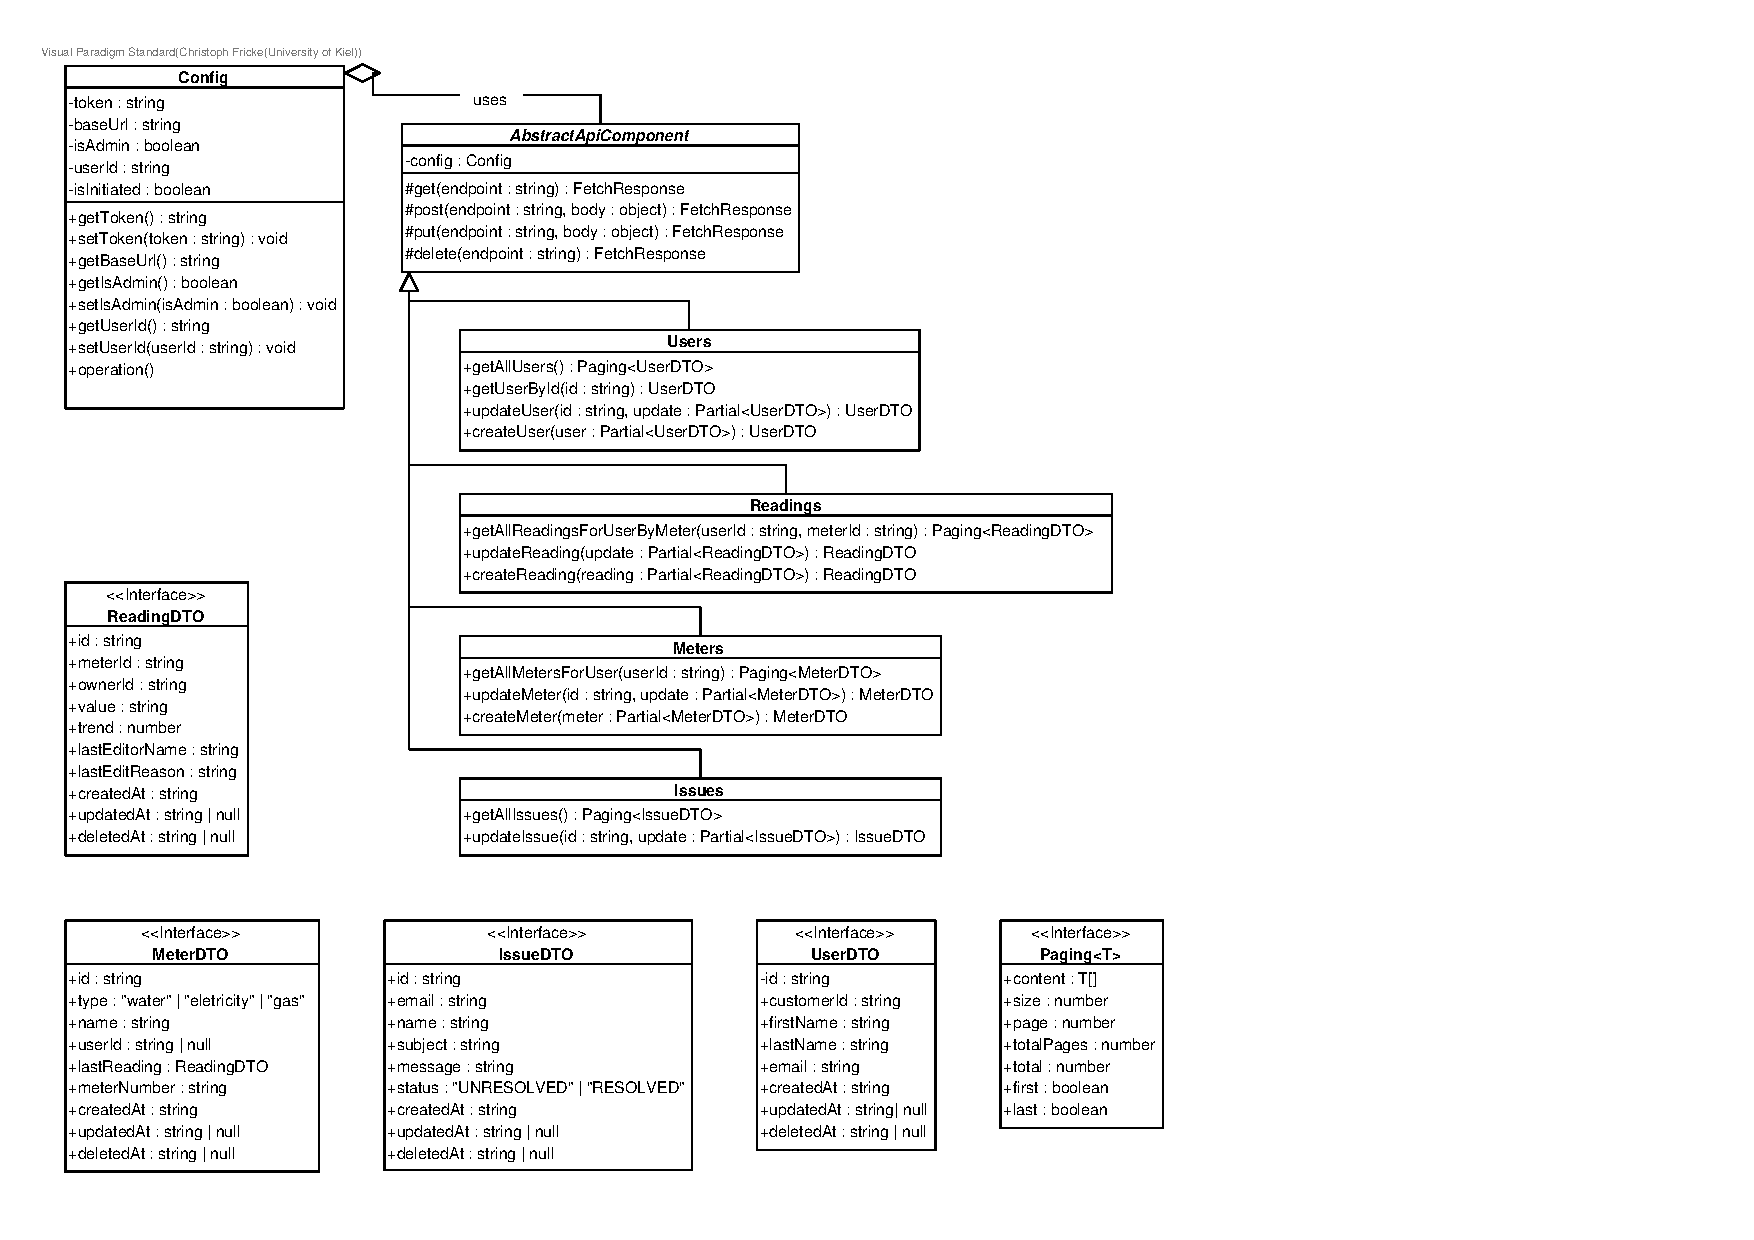
\includegraphics[scale = 0.9]{./img/Diagrams/api-classDiagram}
	\caption{Klassendiagramm - API Abstraction}
\end{figure}
\newpage

\textbf{Beschreibung zum obrigen Klassendiagramm - API Abstraction.} \\ \\
Die verschiedenen DTO Interface sind Datentypen welche über die REST-Endpunkten verschickt werden. Sie dienen als Datentyp für Javascript Objekte in Typescript. In der API-Abstraction halten wir eine eigene Config-Klasse, damit Komponenten welche die Abstraction benutzen, nicht bei jedem Aufruf den Token und die Base-URL mitgeben müssen. Dadurch muss die Config nur einmal initialisiert werden, sobald der Benutzer die Website lädt. \\ \\
Eine Abstrakte Klasse stellt konfigurierte Netzwerkfunktionen für die spezialisierten Klassen zur Verfügung, sodass die Methode zum erstellen von Netzwerk Anfragen (fetch oder axios) leichter ausgetauscht werden kann. \\
Die spezialisierten API Componenten + Config sind Singletons. Eine index Datei in den API Package exportiert für
jede Klasse ein Object wodurch auf einfache Art und Weise ein Singleton Pattern in JS realisiert werden kann.
Zum Testen kann weiterhin die Klasse importiert werden, sodass z.b. von der Config in jeden Test ein neues
Objekt verfügbar ist. Dieses Verhalten wäre auch durch Mocking erreichbar, ist jedoch aufwendiger umzusetzen und erzeugt mehr Overhead. \\

\begin{table}[h]
	\centering
	\begin{tabularx}{\textwidth}{X X}
		\rowcolor[HTML]{C0C0C0} 
		\textbf{Klassenname} & \textbf{Aufgabe} \\
		Config& Speichert API Access Informationen wie Token und Base-URL. Auf diese kann nicht zugegriffen werden, bevor die Config initialisiert wurde.  \\
		\rowcolor[HTML]{E7E7E7} 
		AbstractApiComponent & Stellt konfigurierte Netzwerkfunktionen für die spezialisierten Klassen zur Verfügung. \\
		Users & Beinhaltet Funktionen um auf die Rest-Endpunkte zuzugreifen, welche inhaltlich zu den Benutzern gehören. \\
		\rowcolor[HTML]{E7E7E7} 
		Readings & Beinhaltet Funktionen um auf die Rest-Endpunkte zuzugreifen, welche inhaltlich zu den Zählerstände gehören. \\
		Meters & Beinhaltet Funktionen um auf die Rest-Endpunkte zuzugreifen, welche inhaltlich zu den Zählern gehören. \\
		\rowcolor[HTML]{E7E7E7} 
		Issues & Beinhaltet Funktionen um auf die Rest-Endpunkte zuzugreifen, welche inhaltlich zu den Tickets gehören. \\
	\end{tabularx}
	\caption{Klassenbeschreibung - API Abstraction}
	\label{table:klassenbeschreibung-api Abstraction}
\end{table}


\begin{figure}[H]
	\hspace{-3cm}
	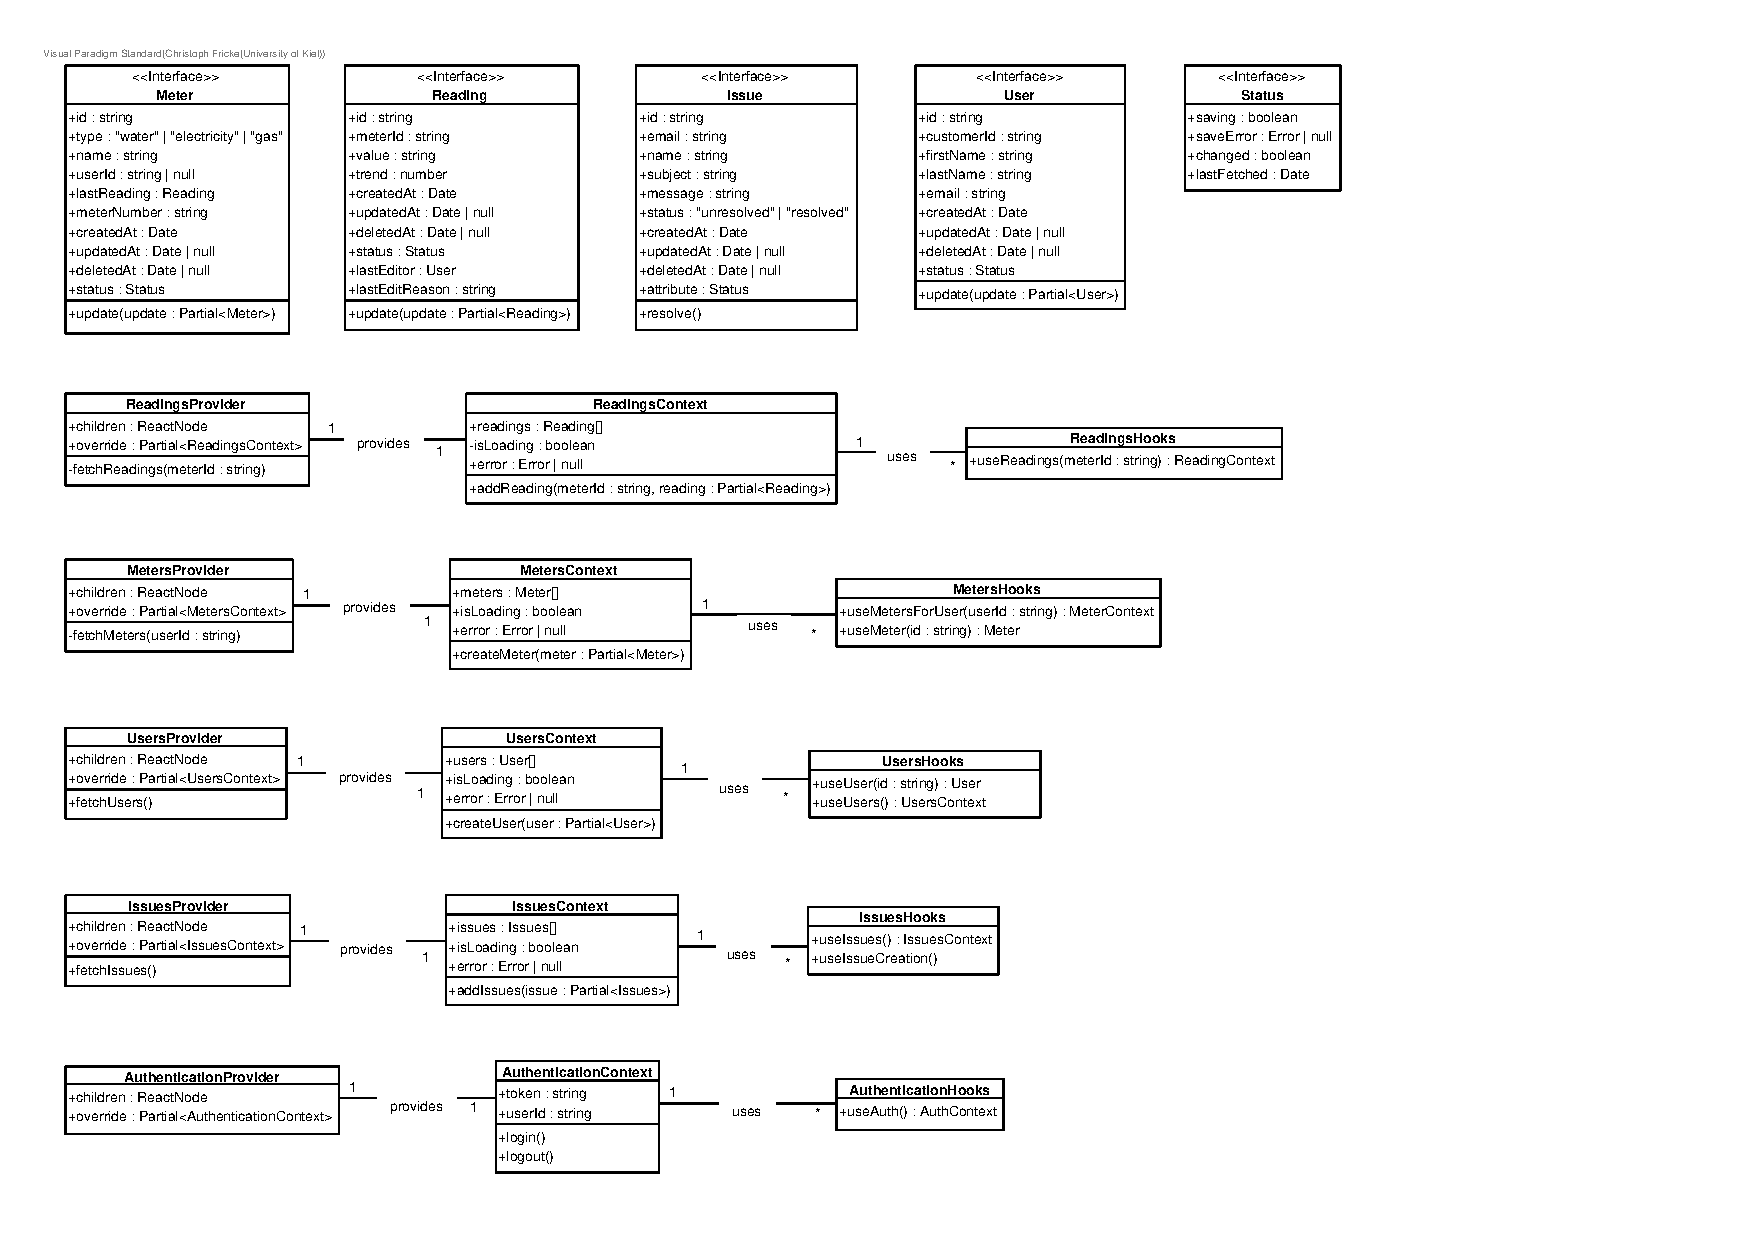
\includegraphics[scale = 0.9]{./img/Diagrams/providers-classDiagram}
	\caption{Klassendiagramm - Provider}
\end{figure}
\newpage

\textbf{Beschreibung zum obrigen Klassendiagramm - Provider.} \\ \\
Für das Klassendiagramm für die Provider ist es wichtig \href{https://reactjs.org/docs/context.html}{React Context} zu verstehen.  Der Override in den Providern erlaubt es uns den Context in Tests auszutauschen. Dadurch können Components, deren Kinder oder diese selber einen Access Hook  benutzen, 
getestet werden, ohne das der Hook gemockt werden muss. \href{https://reactjs.org/docs/hooks-intro.html}{Hooks} sind eine React-Funktionalität um Logik innerhalb von Componenten zu abstrahieren und wiederzuverwenden. Ein Context wird hier als Klasse dargestellt. In Wahrheit ist es aber ein Objekt, 
welches von React verwaltet wird. Dadurch werden konsumierende Components bei Updates automatisch neu gerendert. Das Ganze ist vergleichbar mit einem Observer Pattern. \\
Die Hook Klassen existieren nur im Diagramm. Im Quellcode sind es nur die aufgelisteten Hooks, welche von den UI Components benutzt werden können um Zugriff auf die Contexte zu bekommen. Die Hooks dienen damit als Fassade, sodass die React Contexte auch durch Redux für das globale State Management ersetzt werden könnten.
Provider Components bringen die verschiedene Contexte in den React-Tree, damit diese für die Hooks in den UI Components zur Verfügung stehen.\\
Die Interface welche im Context gehalten werden, sind erweiterte DTO interface welche zusätzliche interne Informationen speichern.

\begin{table}[h]
	\centering
	\begin{tabularx}{\textwidth}{X X}
		\rowcolor[HTML]{C0C0C0} 
		\textbf{Klassenname} & \textbf{Aufgabe} \\
		*Context & Conxtexte stellen ihren zugehörige Informationen global zur Verfügung.  \\
		\rowcolor[HTML]{E7E7E7} 
		*Provider & Die Provider rendern ihren zugehörigen Context in den React-Tree. \\
		*Hooks & Hooks sind Zugriffsfunktionen als Fassade für die zugehörigen Contexte, damit die Componenten nicht direkt auf den Context zugreifen. \\
	\end{tabularx}
	\caption{Klassenbeschreibung - Provider}
	\label{table:klassenbeschreibung-provider}
\end{table}
\newpage

\begin{figure}[H]
	\hspace{-3cm}
	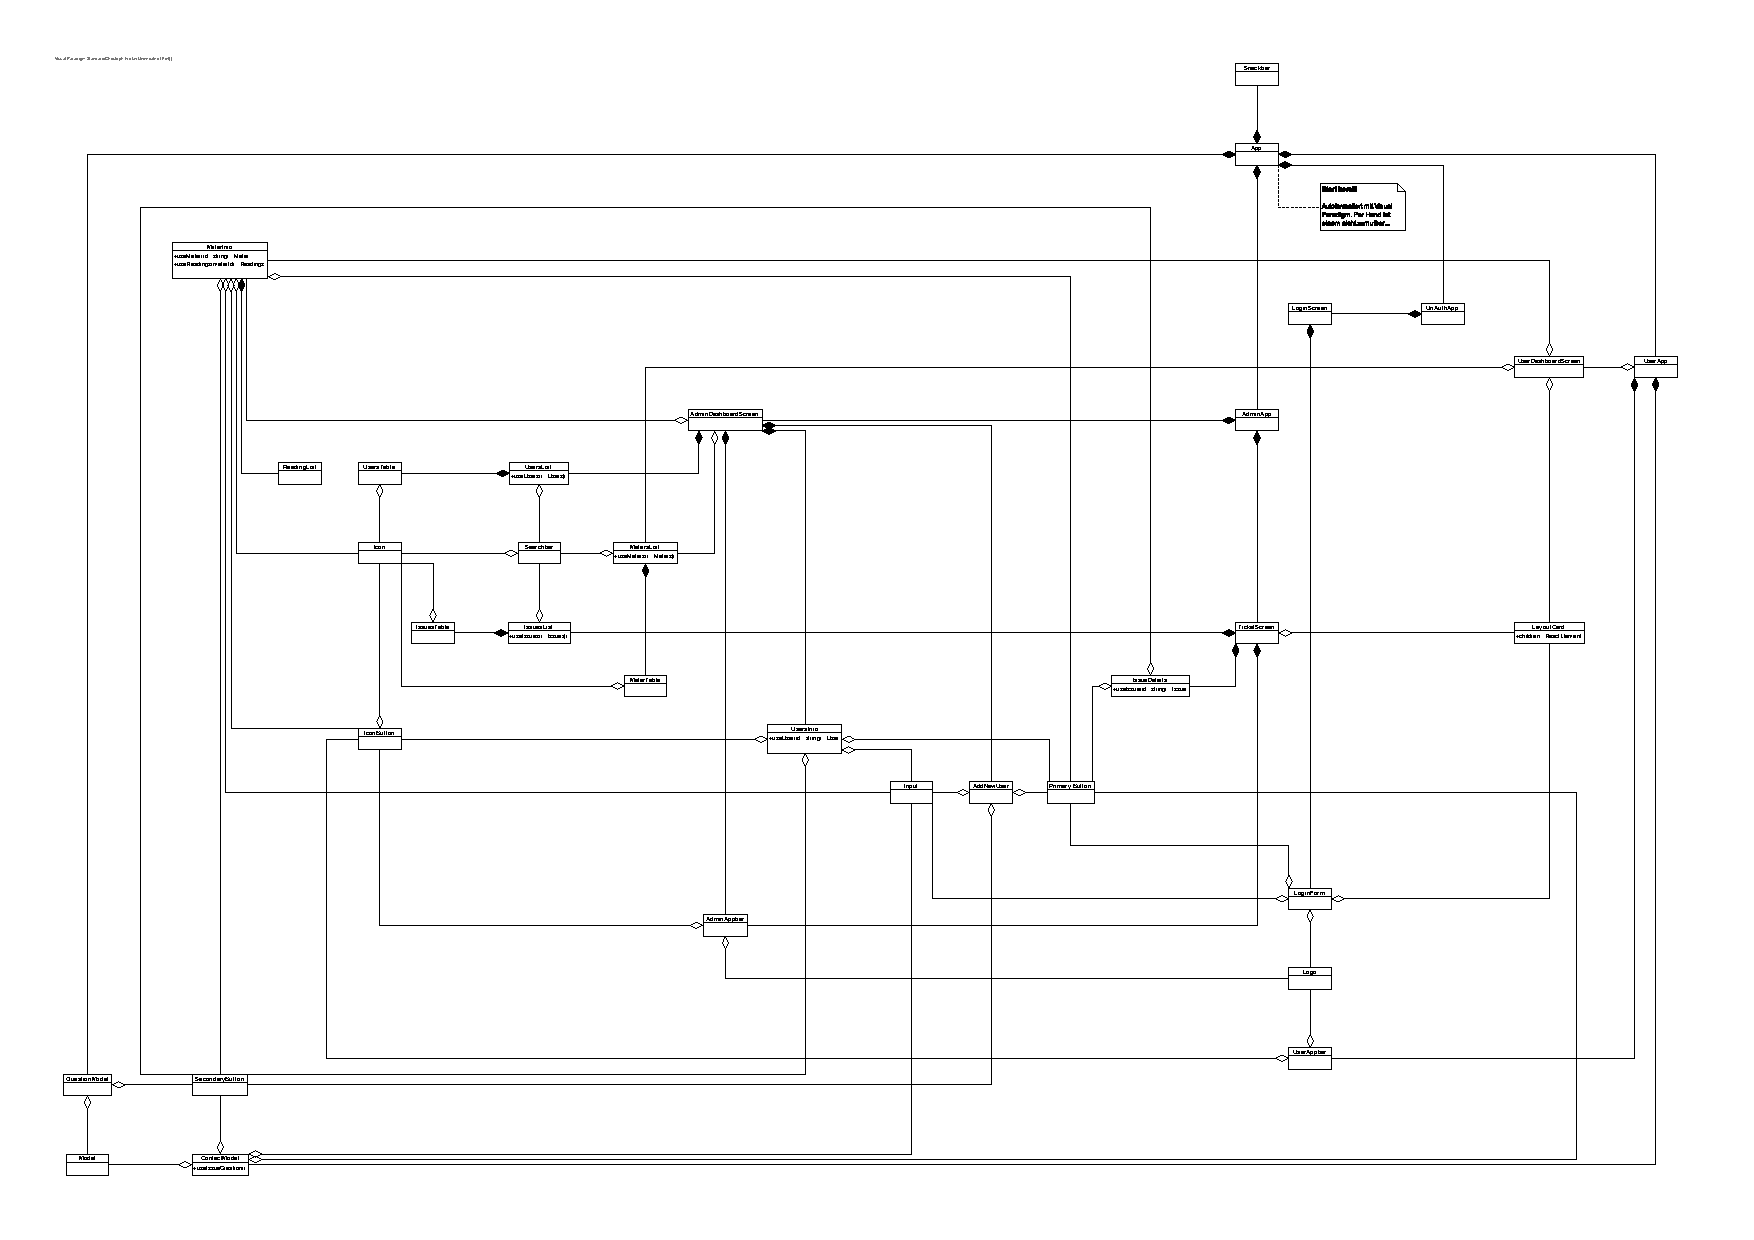
\includegraphics[scale = 0.9]{./img/Diagrams/web-class}
	\caption{Klassendiagramm - Benutzeroberfläche Componenten}
\end{figure}
\newpage

\textbf{Beschreibung zum obrigen Klassendiagramm - Benutzeroberfläche Componenten} \\ \\
Alle Klassen aus dem Diagramm sind \href{https://reactjs.org/docs/components-and-props.html}{React-Componenten}. Damit es übersichtlicher ist, haben wir die Properties und internen State sowie die Kardinalitäten der Associationen rausgelassen und nur Hooks aus der Provider-Schicht hinzugefügt wo wir vermuten auf den globalen State zuzugreifen. \\ \\
Allgemein bestehen die Benutzeroberflächen aus Kompositionen von UI Componenten welche von React in den HTML-DOM gerendert werden. 
 
\begin{table}[h]
	\centering
	\begin{tabularx}{\textwidth}{X X}
		\rowcolor[HTML]{C0C0C0} 
		\textbf{Klassenname} & \textbf{Aufgabe} \\
		App & App ist die Hauptkomponente welche in den HTML-DOM gerendert wird. Basierend auf den Status des Benutzers, rendert diese entweder die User-App, die Admin-App oder die Unauth-App. \\
		\rowcolor[HTML]{E7E7E7} 
		Layout Card & Die Layout Card rendert eine weiße Box welche als Container für ihre inneren Componenten dient.  \\
		Snackbar & Die Snackbar sind kleine Pop-up Benachrichtigungen welche dem Benutzer Statusmeldungen mitteilen.  \\
		\rowcolor[HTML]{E7E7E7} 
		UsersList & Die UsersList rendert eine Liste mit Suchbar von allen Benutzern. \\
		MetersList & Die MetersList rendert eine Liste mit Suchbar von allen Zählern eines Benutzers. \\
		\rowcolor[HTML]{E7E7E7} 
		IssuesList & Die IssuesList rendert eine Liste mit Suchbar von allen Tickets.\\
		UsersInfo & Enthält Informationen über die Benutzer und die Möglichkeit diese zu editieren. \\
		\rowcolor[HTML]{E7E7E7} 
		IssueDetails & Enthält eine Detaillierte Ansicht über ein Ticket und Interaktions möglichkeiten.\\
		MeterInfo & Enthält Informationen über einen Zähler und seine Zählerstände.
	\end{tabularx}
	\caption{Klassenbeschreibung - Benutzeroberfläche Componenten}
	\label{table:klassenbeschreibung-ui}
\end{table}
